% !TEX root = cha-approach.tex
\documentclass[../../main.tex]{subfiles}

\begin{document}

\section{Challenges \& Enhancements}
In this section we present some challenges encountered during the development of our approach, how we solved them, and the specific enhancements made to adapt the WFC algorithm to software visualization.

\subsection{Managing the Exploding Number of Tiles}
A major challenge when scaling our approach to larger systems was the explosion in the number of tiles. In a naive implementation, each path requires dedicated tiles that encode the path ID on its edges, even if they were visually identical. We initially created 11 dedicated tiles for each unique path ID, plus additional tiles for every pair of overlapping paths. However, this caused the tileset size to explode as soon as we targeted larger software systems. Since the propagation phase is the most computationally intensive part of WFC, this naive design made the approach computationally infeasible even for medium-sized systems.

To address this issue, we introduced a \emph{placeholder tile system}. At initialization, every grid cell contains the empty tile and a fixed set of 14 generic path tiles, where path identities are represented by placeholders rather than concrete IDs. This strategy bounds the candidate tileset of each cell to 15 tiles regardless of the total number of paths, keeping constraint propagation tractable. Concrete path IDs are originally embedded only in the edges of the class nodes placed on the grid. As path cells collapse, path ID information propagates from cell to cell, resolving placeholders into concrete tiles on the fly.

This works because our cell selection strategy targets the cell with the maximum entropy (\subsecref{subsec:wassis_observation_phase}), so cells adjacent to already established paths are prioritized. However, when multiple candidate cells share the exact same entropy, WFC may collapse a path cell that is not yet connected to a resolved neighbor, leaving its path ID temporarily unknown. This is represented as a black path, an example is shown in \figref{fig:pathID_resolution} (left).

To handle these cases, we perform a path ID propagation step immediately after collapsing a cell and before standard WFC propagation begins. The resolution process operates as follows:

\begin{enumerate}
    \item Once a cell $C$ collapses into a resolved path tile (a tile without placeholders), it is added to a queue to propagate the information to its neighbors.
    \item While the queue is not empty, WFC checks the adjacent collapsed neighbors $N$. If a neighbor $N$ contains a placeholder tile, it resolves $N$ into a concrete path tile using the ID information from $C$.
    \item If neighbor $N$ successfully resolves into a concrete tile, it is added to the queue to further resolve its neighbors, if necessary.
    \item After updating placeholder tiles, WFC verifies that touching edges between adjacent resolved tiles match. If an edge mismatch is detected, a contradiction is signaled.
\end{enumerate}

An example of this process is illustrated in \figref{fig:pathID_resolution}. In the state on the left, a path segment has been collapsed using placeholder tiles (shown as black paths) because its specific path ID was temporarily unknown. In the next step, when the cell highlighted with the green border collapses into a resolved tile (a T-junction connected to the main path), it propagates the information about the concrete path ID to the path segment, immediately resolving it into concrete tiles. 

Once all placeholders are resolved, WFC performs standard propagation from the collapsed cell. This ensures that the new constraints are propagated to neighboring cells.

\begin{figure}[htbp]
    \centering
    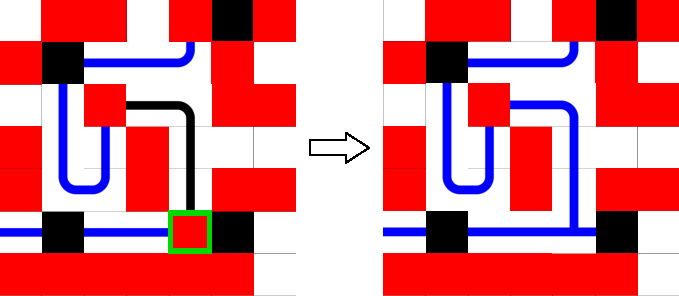
\includegraphics[width=0.9\linewidth]{figures/approach/pathID_resolution}
    \caption{Resolution of path ID placeholders during generation.}
    \label{fig:pathID_resolution}
\end{figure}

\subsection{Guiding Paths Towards Their Targets}

A problem with WFC is that, even when classes that should be connected are placed close to each other using MDS, path tiles are still selected through a weighted random choice. Therefore, there is no guarantee that a path will be generated towards the class or path where it should connect. The path may instead grow in a different direction and fail to reach its target. While this works for very small examples (\eg 5 classes), it becomes impractical for larger software systems.

To address this problem, we implemented two main strategies:

\begin{itemize}
    \item \textbf{Directional Path Exits:} Path exits are fixed for each class before the WFC generation starts. Their direction is chosen based on the position of their target.
    \item \textbf{Dynamic Tile Weighting:} Path tiles are not selected completely randomly. Taking inspiration from the approach proposed by Sandhu~\etal~\citebibliography{Sandh2019a}, the weights of tiles that move a path towards its target are temporarily boosted.
\end{itemize}

\paragraph{Path Exits}

Before the WFC generation starts, path exits (and entries) are assigned to the borders of each class with concrete path IDs. This fixed assignment is necessary because, as described in \subsecref{subsec:wassis_observation_phase}, the generation process starts directly from the classes. Consequently, when a path reaches its target class, it cannot connect to any cell on the class border, but it must connect to the designated entry point. 

To determine these exit points, we compute the centroid of all classes sharing that path. The path IDs are then assigned to the edges of the class cells that point towards this centroid. In this way, paths are more likely to start in the direction of their target.

\paragraph{Path Target}

When a cell that must be a path is selected for collapse, the direction towards its target is known. We temporarily increase the weights of the tiles that continue the path in that direction. This increases the probability of selecting a tile that moves the path closer to its target.

This strategy takes advantage of our observation phase (\subsecref{subsec:wassis_observation_phase}), where path cells are collapsed before empty cells. In addition to the path ID, we can pass the target information associated with each path ID to the next path cells.

\noindent We support three strategies for determining the target of a path:

\begin{itemize}
    \item \textbf{\textbf{Centroid}:} The target is the centroid of all classes sharing the same path ID.
    \item \textbf{\textbf{Nearest Class}:} The target is the nearest class sharing the same path ID.
    \item \textbf{\textbf{Random}:} No target direction is used and the tile weights are not boosted.
\end{itemize}

Note that ``black paths'' (\figref{fig:pathID_resolution}) do not have information about neither the path ID nor its target. Therefore, they are generated completely randomly.

\subsection{Reducing the Number of Crossings}
Our approach does not explicitly minimize path crossings through a dedicated optimization step. Instead, crossings are naturally minimized during path generation by assigning them a weight of zero (\subsecref{subsec:wassis_observation_phase}). As a result, Wave Function Collapse introduces crossing tiles only when constraint propagation eliminates all the alternatives, ensuring they appear only when strictly necessary to complete a path.

\subsection{Backtracking Strategies}
\label{subsec:backtracking_strategies}

The standard Wave Function Collapse implementation~\citeonline{Gumin2016wfc} does not support backtracking and restart from scratch when a contradiction occurs. Inspired by the work of Karth~\etal~\citebibliography{Karth2022a}, we introduced backtracking into our approach to improve the success rate of the generation.

When a contradiction occurs, the generation process follows this recovery process:

\begin{enumerate}
    \item \textbf{Local Backtracking:} The algorithm goes back to a previous decision using one of the strategies described below, up to a fixed number of backtracks.
    \item \textbf{Restart with Same Placement:} If local backtracking fails, the generation restarts using the same grid size and classes placement. This is repeated for a fixed number of attempts.
    \item \textbf{Restart with Same Grid Size:} If the previous attempts fail, the generation restarts with the same grid size but computes a new class placement. This is also repeated for a fixed number of attempts.
    \item \textbf{Grid Expansion:} If all previous attempts fail, the grid size is increased and the generation starts again from the beginning.
\end{enumerate}

The backtracking workflow is shown in \figref{fig:backtracking_workflow}.

\begin{figure}[ht]
    \centering
    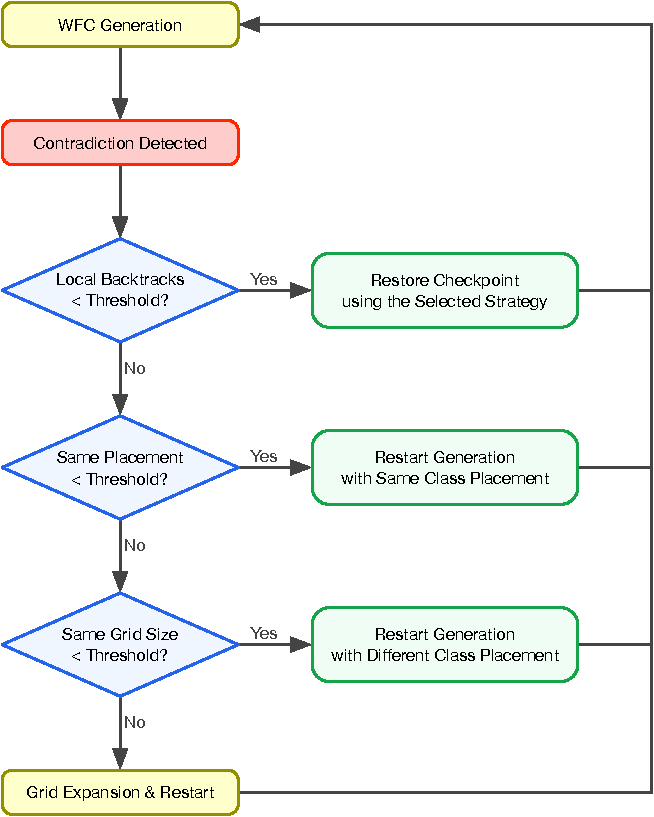
\includegraphics[width=0.71\linewidth]{figures/approach/backtracking_workflow}
    \caption{Backtracking workflow}
    \label{fig:backtracking_workflow}
\end{figure}

We implemented five strategies for backtracking:

\begin{itemize}
    \item \textbf{Fixed Number of Steps:} Goes back a fixed number of steps from the current state. If this goes beyond the beginning of the generation, the process restarts from the beginning. 
    \item \textbf{Percentage of Steps:} Goes back by a fixed percentage of the steps performed so far. If this goes beyond the beginning of the generation, the process restarts from the beginning. 
    \item \textbf{Many Possible Tiles:} Goes back to a checkpoint saved before a cell with many possible tiles was collapsed. The user defines a minimum number of possible tiles as a threshold for saving the checkpoint.
    \item \textbf{Similar Tile Weights:} Goes back to a checkpoint saved before a cell was collapsed when its possible tiles had similar weights. The user defines the percentage of tiles to consider and the maximum allowed difference between their weights, expressed as a percentage. 
    \item \textbf{Restart:} Clears the current grid and starts the generation again from the beginning.
\end{itemize}

When a checkpoint is restored, the cell is brought back to the state it had immediately before the original collapse. If the tile originally selected was a path tile, it is removed from the cell's possible tiles before the cell is collapsed again. This prevents WFC from making the same choice and allows it to explore a different alternative.

\subsection{Path Optimization}
\label{subesc-approach:path_optimization}

WFC generates valid paths between classes, but these paths are not always optimal. Since WFC uses local rules and random tile selection, despite weights boosting, paths may contain unnecessary deviations. To reduce these detours, we added an optional \textit{Path Optimization} step after WFC generation. The optimization removes the tiles of a selected path and rebuilds the path using Dijkstra's algorithm:

\begin{itemize}

\item \textbf{Direct Connections:} If the path connects two classes, Dijkstra's algorithm finds the shortest path between their border nodes.

\item \textbf{Merged Paths:} If a path connects multiple classes, the algorithm builds a merged path connecting all of them. It works as follows:

    \begin{enumerate}
        \item \textit{Backbone Creation:} Dijkstra's algorithm is used to find the shortest path between every pair of classes. The longest path is chosen as the backbone.
        \item \textit{Virtual Node Target:} Each remaining class is connected to the closest node of the backbone using the shortest path.
        \item \textit{Backbone Expansion:} After a class is connected, the new branch of the path is added to the backbone. The remaining classes can connect to both the original backbone and the new branches.
    \end{enumerate}

\end{itemize}

Finally, the selected cells are converted into path tiles, while the others into empty tiles.

\end{document}